\section{Implementation, independent checks, and measured performance}
\label{sec:experiments}

\subsection{Evidence and timing conventions}

The proofs establish asymptotic claims for their stated input models.
Independent finite checks test whether the implementation realizes those
models. Timings answer a narrower question about the cost of these particular
implementations in the recorded environment. These three forms of evidence
are reported separately.

The recorded runtime was Python 3.12.14 on Linux x86\_64, kernel 6.18.44,
with glibc 2.39. The optional native geometry audit used the Regina 7.4.1
Python distribution; its library version string reports 7.4. Computations
ran in a shared environment without CPU isolation. Absolute elapsed times
should therefore be treated as descriptive measurements, not portable
performance predictions. In particular, repeated geometry runs varied under
shared load. The final recorded JSON files, rather than earlier working
measurements, supply every table below.

The arithmetic measurements use three repetitions per input and include
certificate generation and the optimizer's independent certificate check.
Normal extraction uses five repetitions on the layered-torus sequence and
seven for fixed triangulation size. Fixtures are built before these timed
regions. No expanded surface or native component computation is called on
the large normal-coordinate cases.

The scalar benchmark uses seven randomized paired rounds. Each arm has a
fresh state, an untimed warm-up, and between one and five calls per round,
with batch size recorded in the data. A/A controls run the reference twice.
A reported ratio is
\[
 \operatorname{median}_{j=1}^7\frac{T_{\mathrm{reference},j}}
                                      {T_{\mathrm{variant},j}},
\]
so values greater than one favor the variant. This differs in general from
the ratio of the two separately reported median times. Exact output
comparisons and scalar-locality certificate audits are outside these timed
regions. No confidence interval or natural-knot speedup is inferred from a
few percent of timing variation.

\subsection{Arithmetic correctness and binary-size stress cases}

The standalone arithmetic tests use exhaustive enumeration of the original
variables as the reference, not the parameterization returned by the new
solver. The exhaustive and seeded comparisons total:

\begin{center}
\small
\begin{tabular}{lr}
\toprule
Independent arithmetic comparison & Cases\\
\midrule
Scalar merges, $m\le48$ & 38\,024\\
Two-coordinate merges, $m\le8$ & 8\,772\\
Two-generator scalar cosets, $m\le10$ & 3\,025\\
Scalar congruences, $m\le24$ & 4\,900\\
$2\times2$ systems, $m\le4$ & 4\,890\\
One-variable one-seam families, $m\le6$ & 2\,275\\
Seeded dense random families & 2\,000\\
\textbf{Total} & \textbf{63\,886}\\
\bottomrule
\end{tabular}
\end{center}


Additional tests cover empty parameter and holonomy dimensions, modulus one,
cooperative cancellation, malformed input, and deliberately corrupted
certificates. The corresponding thirteen \code{unittest} methods are
included in the integrated suite. The verifier can be run without calling
the optimizer or trusting a supplied kernel basis.

\begin{center}
\small
\begin{tabular}{lrrrr}
\toprule
Family & Modulus bits & $n/q/\beta$ & Min. & Seconds\\
\midrule
$2+z$, no seams & 2\,648 & 1/0/1 & 1 & 0.000081\\
$2+z$, no seams & 42\,353 & 1/0/1 & 1 & 0.008106\\
$2+z$, no seams & 169\,409 & 1/0/1 & 1 & 0.191455\\
Dense constrained & 131 & 24/12/7 & 6 & 0.019229\\
Dense constrained & 515 & 24/12/7 & 6 & 0.039649\\
Dense constrained & 2\,051 & 24/12/7 & 6 & 0.231718\\
Dense constrained & 8\,195 & 24/12/7 & 6 & 2.446944\\
\bottomrule
\end{tabular}
\end{center}


Here $n/q/\beta$ gives the variable, constraint, and holonomy dimensions.
For the last one-parameter row, $m=6^{65536}$ has 169,409 bits. The returned
witness is $z=3^{65536}$, and exactly seventeen saturation gcds are used.
The algorithm represents no individual sheets and enumerates no parameter
tuples. Its work is controlled by binary length, not by the astronomical
integer value of $m$.

The dense stress families have a deliberately planted exact optimum six.
For a seeded dense matrix $A$, a feasible hidden vector has every coordinate
divisible by six. The first six holonomy rows are $A_j+6R_j$, and the last
holonomy is the constant six. On the feasible locus all coordinates are
multiples of six, and the last coordinate forces their gcd with $m$ to be
six. The returned certificates have six nonzero dual entries. This design
provides a known independent answer while exercising dense congruence
elimination and nontrivial dual certificates; it is not presented as a
sample of difficult knot exteriors.

\subsection{Surface-family compilation and query boundaries}

The geometric wrapper has nineteen regression methods. Its seeded test
constructs 120 families, of which 51 are feasible and 69 are infeasible.
It examines 1,337 original parameter assignments: 437 satisfy the seams,
and 900 fail them. For each feasible assignment, a direct disjoint-set
calculation on patch--sheet pairs agrees with the compiled component count.
This reference does not use spanning-tree potentials or the compiled loop
list. Every family's minimum and feasible-assignment count agree with the
literal results, and both kinds of certificate verify.

Targeted cases check a tree edge traversed backwards, reversal of a seam,
nonorientable peripheral squares, both base-boundary degrees, and gluing
that connects locally disconnected covers. The emitted large-integer JSON
certificates also survive a serialize--parse--verify round trip. This last
check is material: a verifier that accepts a large integer in memory but
rejects its documented hexadecimal transport is not a usable artifact
verifier. The wrapper decodes only documented certificate integer fields;
it does not interpret unrelated metadata as mathematics.

A separate check of Theorem~\ref{thm:peripheral-hardness} uses the maintained
surface-cover classifier to inspect the full lifted-boundary profiles for
all 351 assignments of three graph families:

\begin{center}
\small
\begin{tabular}{lrrr}
\toprule
Graph & Assignments & Globally connected & \shortstack{All designated\\boundaries connected}\\
\midrule
$K_3$ & 27 & 24 & 6\\
$K_4$ & 81 & 78 & 0\\
$C_5$ & 243 & 240 & 30\\
\bottomrule
\end{tabular}
\end{center}

These checks are distinct from the 63,886 arithmetic cases. The $K_4$
example makes the interface boundary concrete: a family can have many
globally connected members and no member satisfying all requested
peripheral connectedness conditions.

\subsection{Normal-coordinate extraction: exact geometric and native audits}

The local geometric oracle realizes triangle and quadrilateral discs by
rational barycentric levels and sorts the actual face intersections.
Its 1,537 cases cover all 24 vertex permutations, all four source faces,
and all absent/active quadrilateral combinations on each side. The two
methods agree on 9,771 individual disc identifications and 4,850 prism-gap
identifications. The latter include 591 reflected bands, which exercise
the otherwise easy-to-miss $-1$ in the reflected gap map.

A separate Regina comparison covers 807 small normal-surface inputs and
1,537 component coordinate/topology records, including 92 nonorientable
and 274 closed components. It checks full component-coordinate multisets,
Euler characteristics, orientability, and boundary counts. Scalar multiples
of one-sided surfaces and compatible nonextreme sums are included.
Eight additional package tests exercise the command-line interface,
callbacks, schema errors, matching failures, empty surfaces, and binary
coordinate transport. These finite comparisons support the implementation;
they do not replace the extraction proof.

For the Fibonacci meridian family inherited from the earlier certificate
report, the final measurements are:

\begin{center}
\small
\begin{tabular}{rrrrrrr}
\toprule
$t$ & Coordinate bits & Surface & Prism & Contacts & Residue & ms\\
\midrule
8 & 108 & 44 & 34 & 14 & 32 & 0.833\\
16 & 342 & 92 & 82 & 30 & 64 & 1.679\\
32 & 1\,214 & 188 & 178 & 62 & 128 & 3.533\\
64 & 4\,554 & 380 & 370 & 126 & 256 & 7.162\\
128 & 17\,635 & 764 & 754 & 254 & 512 & 15.081\\
256 & 69\,391 & 1532 & 1522 & 510 & 1024 & 20.934\\
512 & 275\,267 & 3068 & 3058 & 1022 & 2048 & 57.337\\
1024 & 1\,096\,505 & 6140 & 6130 & 2046 & 4096 & 115.382\\
\bottomrule
\end{tabular}
\end{center}


``Coordinate bits'' is the sum of the binary coordinate lengths, with one
bit charged for zero; it is not the maximum coordinate length. ``Surface''
and ``Prism'' count face-pairing bands, ``Contacts'' counts the exceptional
prism-to-residue contacts, and ``Residue'' counts local residual cells.
At $t=128$ the input represents exactly
\[
 2\,791\,715\,456\,571\,051\,233\,611\,642\,548
\]
normal discs, but only 764 surface bands and 754 prism bands are produced.
For two fixed tetrahedra with 65,536-bit multiplicities, there remain ten
stacks, four surface bands, and four prism bands; the recorded seven-run
median is 0.000600 seconds. These are representation and extraction
measurements. They do not include general orbit reduction, parallelity
bundle recognition, or a complete hierarchy iteration.

\begin{figure}[tb]
\centering
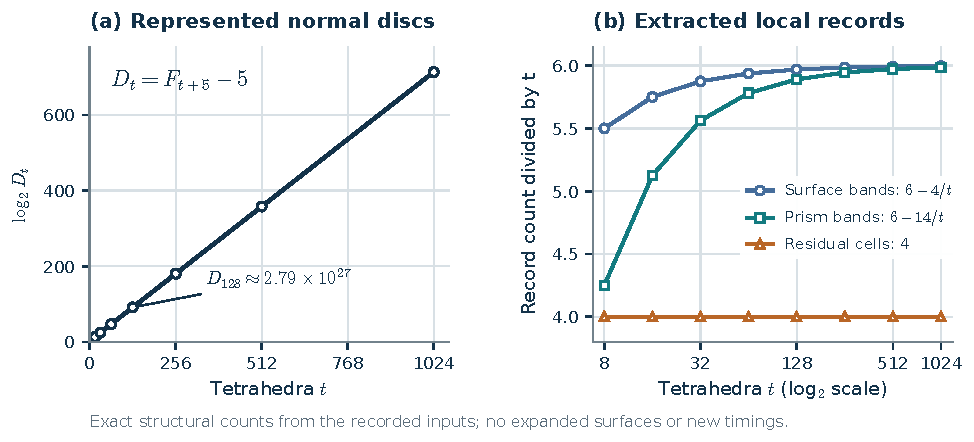
\includegraphics[width=\linewidth]{figures/normal_extraction_scaling.pdf}
\caption{Exact structural counts for the inherited Fibonacci meridian
family, at the recorded values $t=8,\ldots,1024$. The normal-disc count
is $D_t=F_{t+5}-5$. Its binary logarithm grows linearly with $t$ in
panel (a), while panel (b) shows bounded numbers of extracted records per
tetrahedron. The horizontal axes use different scales, as labelled.
These are count data, with no fitted running-time exponent.}
\label{fig:normal-scaling}
\end{figure}

\subsection{Attached copies: exact equation savings and a crossover}

The attached-copy benchmark compares the modified backend with the pinned
\code{scalar_split.py}; both use the same remaining dependency modules.
The measured region is recursive scalar compression followed by component
sharing. Fixture construction is outside the timed region.

\begin{center}
\small
\begin{tabular}{rrrrrrr}
\toprule
$r$ & Old equations & Inherited & Old solves & New & Ratio & A/A\\
\midrule
4 & 58 & 32 & 3 & 1 & 0.848 & 1.027\\
8 & 406 & 128 & 7 & 1 & 1.099 & 1.051\\
12 & 1\,298 & 288 & 11 & 1 & 1.252 & 1.013\\
16 & 2\,990 & 512 & 15 & 1 & 1.468 & 0.999\\
24 & 9\,798 & 1\,152 & 23 & 1 & 1.759 & 0.989\\
\bottomrule
\end{tabular}
\end{center}


The equation counts are the exact values proved in
Section~\ref{sec:inheritance}. At $r=16$, repeated solves construct 2,990
nonzero equations across fifteen commutant computations, while inheritance
constructs 512 equations in one computation. Candidate order and accepted
split witnesses agree. The 1.468 paired ratio reflects an actual measured
benefit. At $r=4$, the ratio 0.848 instead shows the cost of transport and
canonicalization exceeding the saving.

The $r=24$ experiment raises the backend caps: its 72 objects and 1,728
scalar variables exceed the default limits, and its 23 splits exceed the
default split budget of sixteen. It is a controlled scaling experiment,
not a claim about behavior under default caps. The $r\le16$ rows fit the
default object and variable limits. Neither the exact cubic-to-quadratic
equation reduction nor the measured ratios establish an analogous total
bit-time exponent for arbitrary complexes.

\subsection{Field algebras: identify the work that actually matters}

For the dense two-field family, the reference is the previously supplied
primary-projector policy, with descendant commutants recomputed. This is
a separate reference from the pinned zero-primary Fitting search used for
the preceding table. The new mechanisms are measured independently:

\begin{center}
\small
\begin{tabular}{rrrrrr}
\toprule
$r$ & Inheritance & Local stop & Both & One generator & A/A\\
\midrule
8 & 0.890 & 1.877 & 1.446 & 2.165 & 1.003\\
10 & 0.868 & 2.033 & 1.565 & 2.312 & 1.002\\
12 & 0.895 & 1.935 & 1.489 & 2.229 & 0.985\\
\bottomrule
\end{tabular}
\end{center}


The four variant columns mean general corner inheritance only, direct
saturation-locality stopping only, their ordinary combination, and the
one-generator corner path with locality certification. General inheritance
alone is slower in all three displayed cases. Carrying the full basis is
not the right optimization for these low-dimensional commutative algebras.
The saturated generator exposes the complete algebra and finishes both
local children directly.

For degrees $r=8,10,12$, the old candidate counts are respectively
46, 52, and 58. The one-generator path uses two candidate tests and one
commutant computation, followed by two scalar-locality certificates.
The reference uses three commutant computations. The corresponding paired
ratios are 2.165, 2.312, and 2.229. The $r=12$ root has 1,152 scalar
variables, exceeding the default variable cap, although its 48 objects
fit the default object cap.

The data also retain lower-degree cases and a degree-eight case using only
one elementary change of basis to mix the two blocks. Not every accepted generator saturates the algebra; the latter case
falls back to ordinary inheritance, and direct local stopping is faster.
This is evidence for a cost-aware choice of mechanism, rather than for
turning every optional feature on unconditionally. All these fixtures are
legitimate homogeneous algebraic complexes; no realization as natural knot
scan prefixes is claimed.

\subsection{Natural scans: a useful negative timing result}

Natural examples measure a complete raw Khovanov scan, including scanner
construction, at the same preselected order for every arm. Loading the
input and finding that order are excluded. Homological ranks and the
configured capped decisions are checked independently. The timing table is:

\begin{center}
\small
\begin{tabular}{lrrrrrl}
\toprule
Diagram & Crossings & Old ms & Inherit & One gen. & A/A & Solves\\
\midrule
Trefoil & 3 & 0.319 & 0.961 & 0.958 & 1.003 & 0\,$\to$\,0\\
Conway & 11 & 7.530 & 0.990 & 1.018 & 0.954 & 10\,$\to$\,7\\
Kinoshita--Terasaka & 11 & 8.079 & 1.022 & 1.010 & 1.016 & 9\,$\to$\,6\\
Hard unknot 8 & 8 & 0.732 & 1.001 & 0.993 & 1.002 & 0\,$\to$\,0\\
Stress braid 5/36 & 36 & 457.241 & 1.021 & 0.980 & 1.005 & 5\,$\to$\,5\\
$T(3,5)$ & 10 & 2.917 & 0.998 & 0.994 & 0.982 & 0\,$\to$\,0\\
\bottomrule
\end{tabular}
\end{center}


The final column counts actual commutant computations; for the historical
arm, cache misses equal those computations in these cases. Conway falls
from ten to seven and Kinoshita--Terasaka from nine to six, each using three
inherited child spaces across two Fitting splits. There is a real reduction
in repeated algebra construction. Wall-time inheritance ratios, however,
range only from 0.961 to 1.022, comparable with the control variability.
These measurements support no convincing natural-knot wall-time speedup.
No natural example in this sample activates a primary split, a conclusive
locality certificate, or a monogenic corner. The controlled field gains
must remain separate from claims about the complete recognizer.

\subsection{Integrated regression and the inherited worker correction}

The untouched pinned baseline ran 725 tests: 724 passed and one failed.
The failure in \code{test_communication_retains_input_across_polls} was
reproduced in isolation. Repeating \code{communicate} with the input
removed after a timeout could leave a large worker request only partially
written in the current Python runtime. The earlier projectors archive
already contained a single-submission communication-thread correction.
We copied that correction exactly and attribute it as inherited work.
It is not counted as a new performance theorem or optimization.

The complete staged source bundle then passed \textbf{790 tests}, with no
failures, in 110.342 seconds of reported test-runner time. This includes all
725 baseline methods, twelve restored tests for the inherited primary
projector module, and 53 new arithmetic, family, normal-extraction, and
inheritance/locality methods. Targeted scalar checks also preserve cache,
cap, cancellation, grading, and transactional behavior. The logs are
included, including the original baseline failure; the differing total
suite times are not used as a performance comparison.
